Die in Abbildung \ref{boxplots} dargestellten Boxplots zeigen die Ergebnisse der insgesamt 9 Testreihen aufgeteilt auf die drei Leistungsklassen (LOW, MID, HIGH).


\begin{figure}[h]
\begin{subfigure}[b]{0.5\textwidth}
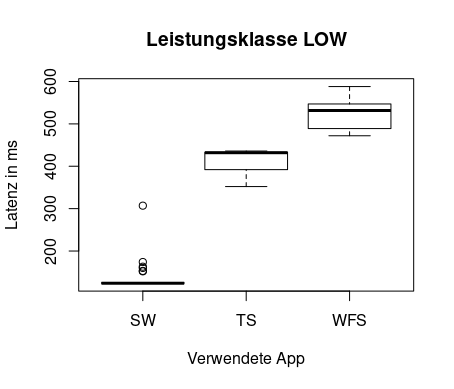
\includegraphics[width=\textwidth]{img/boxplotlow.png}
\end{subfigure}
\begin{subfigure}[b]{0.5\textwidth}
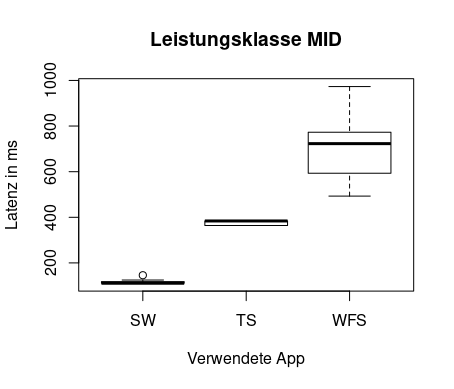
\includegraphics[width=\textwidth]{img/boxplotmid.png}
\end{subfigure}
\begin{subfigure}[b]{0.5\textwidth}
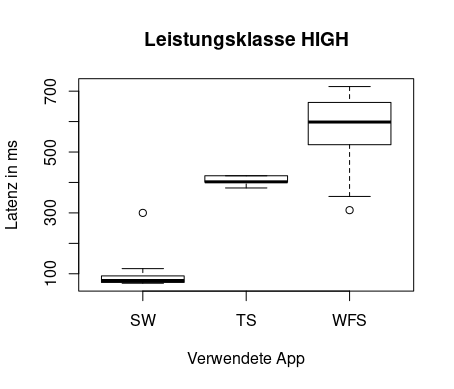
\includegraphics[width=\textwidth]{img/boxplothigh.png}
\end{subfigure}
\caption{Testergebnisse der insgesamt neun Testreihen}
\label{boxplots}
\end{figure}

Nach bloßem Betrachten der Ergebnisse lässt sich die Tendenz verzeichnen, dass bei allen Leistungsklassen SoundWire die geringste Latenz aufweist. Die anschließende statistische Auswertung soll also folgende Hypothesen bestätigen:

\begin{itemize}
\item SoundWire weißt eine geringere Latenz auf als TeamSpeak.
\item SoundWire weißt eine geringere Latenz auf als Wifi Speaker.
\end{itemize}

Die Ergebnisse der einzelnen Testreihen wurden dem Shapiro-Wilk Test unterzogen, um auf Normalverteilung zu überprüfen. Nur die Datenreihe der Leistungsklasse LOW und der App Wifi Speaker verzeichnete dabei einen p-Wert über dem Signifikanzniveau von 0,05 mit einem Wert von 0.06187, wodurch auf eine Normalverteilung geschlossen werden kann. Bei allen anderen Datenreihen ist anzunehmen, dass diese nicht auf einer Normalverteilung basieren.

Die Daten weißen zwar überwiegend keine Normalverteilung auf, allerdings sind in jeder Datenreihe 30 Ergebnisse enthalten. Dadurch ist es möglich, pro Geräteklasse einen T-Test zur Überprüfung der Hypothesen durchzuführen. Dabei ist zu beachten, dass der Datensatz von SoundWire jeweils zweimal verwendet wird. Um das Problem des multiplen Testens zu umgehen, wird das Signifikanzniveau halbiert und somit auf 0.025 gesetzt. Es werden pro Leistungsklasse zwei einseitige T-Tests durchgeführt.

